\documentclass[conference]{IEEEtran}
\IEEEoverridecommandlockouts

% Standard IEEE Conference Packages
\usepackage{amsmath,amssymb,amsfonts}
\usepackage{algorithmic}
\usepackage{graphicx}
\usepackage{textcomp}
\usepackage{xcolor}
\usepackage{booktabs}
\usepackage{cite}
\usepackage{url}
\usepackage{microtype}

\def\BibTeX{{\rm B\kern-.05em{\sc i\kern-.025em b}\kern-.08em
    T\kern-.1667em\lower.7ex\hbox{E}\kern-.125emX}}

\begin{document}

\title{A Cloud-Native, Transformer-Based Battery Management System for Real-Time State of Charge and State of Health Prediction with Digital Twin Monitoring}

\author{
\IEEEauthorblockN{Sudipto Nandi, Adinath, Darshan K, Piyush}
\IEEEauthorblockA{\textit{Faculty Supervisor: Dr. Sangeetha N} \\
\textit{VIT Vellore, India}}
}

\maketitle

\begin{abstract}
Accurate, real-time prediction of State of Charge (SOC) and State of Health (SOH) in lithium-ion batteries is essential for operational safety, performance optimization, and lifespan management across electric vehicles, grid-scale energy storage, and industrial equipment. This paper presents a cloud-native battery management system (BMS) powered by a dual-head, two-layer Transformer encoder architecture exported to the Open Neural Network Exchange (ONNX) format and deployed as a high-throughput, containerized asynchronous API. The model ingests a 32-step sliding window of voltage, current, and temperature telemetry to simultaneously estimate SOC and SOH retention. In reported benchmark evaluations, the Transformer model achieved a coefficient of determination ($R^2$) of 0.985 and a central processing unit (CPU) inference latency ranging between 0.62 and 0.68~ms per window. The production service was integrated with a web-based digital twin monitoring dashboard tracking 200 simulated battery packs across five distinct operational fleets, benchmarked against experimental degradation trajectories from the NASA Ames Prognostics Center of Excellence lithium-ion dataset. The reported benchmarks indicate that the Transformer architecture achieved higher prediction accuracy and lower inference latency than a comparative State-Space Model (SSM/Mamba) baseline on the evaluated platform, demonstrating a viable architectural pathway toward scalable, cloud-connected industrial battery intelligence.
\end{abstract}

\begin{IEEEkeywords}
Battery management systems, state of charge, state of health, transformer neural networks, ONNX Runtime, digital twin, cloud-native inference.
\end{IEEEkeywords}

\section{Introduction}
\IEEEPARstart{L}{ithium-ion} batteries (LIBs) serve as the primary electrochemical energy storage technology across modern sectors, including electric transportation, utility-scale renewable grid balancing, aerospace systems, and automated logistics robotics \cite{Hannan2017, Severson2019}. The operational efficiency, thermal stability, and usable lifespan of LIB packs are governed by a Battery Management System (BMS). Among the critical functions executed by a BMS, the continuous estimation of the State of Charge (SOC) and State of Health (SOH) is paramount \cite{Hannan2017}. SOC quantifies the immediate residual charge relative to usable capacity, acting as an electrochemical fuel gauge. In contrast, SOH reflects irreversible cumulative capacity fade and impedance growth caused by aging phenomena such as solid electrolyte interphase (SEI) layer growth, lithium plating, and active material loss \cite{Plett2004, Saha2007}.

Accurately predicting SOC and SOH under real-world operating conditions presents substantial engineering hurdles. Traditional electrochemical models (such as the pseudo-two-dimensional Doyle--Fuller--Newman formulation) and Equivalent Circuit Models (ECMs) coupled with Extended Kalman Filters (EKF) require extensive parameter identification and struggle to adapt across wide temperature ranges and highly dynamic current discharge cycles \cite{Plett2004, He2011}. Consequently, data-driven machine learning (ML) models have emerged as powerful alternatives capable of mapping nonlinear operational telemetry directly to internal battery states \cite{Chemali2018, Shen2022}. However, practical deployment requires reconciling the tension between predictive accuracy and computational latency while bridging the divide between offline model training and production-ready operational serving \cite{Karnehm2023}.

A notable research gap persists between algorithmic laboratory evaluations and functional, cloud-native battery intelligence architectures. While many studies propose complex neural architectures evaluated on offline test sets, few address the end-to-end integration of time-series neural inference, sub-millisecond CPU model execution, dynamic model hot-swapping, and real-time digital twin fleet visualization within an operational cloud infrastructure. To bridge this divide, this paper describes an end-to-end cloud-native BMS architecture that integrates deep sequence modeling with a resilient, cloud-hosted serving pipeline.

The principal contributions of this work are summarized as follows:
\begin{itemize}
    \item A compact, containerized dual-head two-layer Transformer encoder model exported to ONNX format, optimized for sub-millisecond CPU inference execution (0.62--0.68~ms).
    \item A production-grade FastAPI asynchronous backend service featuring a dedicated model-reload endpoint designed to support model replacement in memory without intentionally terminating the service process.
    \item A web-based digital twin monitoring dashboard providing synchronized telemetry inspection and health diagnostics across five operational environments encompassing 200 simulated battery packs.
    \item Empirical evaluation grounded in publicly available aging data from the NASA Ames Prognostics Center of Excellence (PCoE) lithium-ion battery repository, specifically utilizing reference cells B0005, B0006, B0007, and B0018.
    \item A comparative performance analysis between the dual-head Transformer model and a State-Space Model (SSM/Mamba) sequence baseline across inference latency, parameter efficiency, and prediction accuracy.
\end{itemize}

The remainder of this paper is organized as follows: Section~II reviews relevant literature across battery state estimation, deep sequence modeling, and cloud digital twins. Section~III details the complete system architecture, including model topology, backend API endpoints, and cloud infrastructure. Section~IV delineates the experimental dataset, feature processing, fleet simulation, and evaluation metrics. Section~V analyzes the reported prediction accuracy, latency benchmarks, architectural comparisons, and dashboard performance. Finally, Section~VI concludes the paper and highlights avenues for future inquiry.

\section{Related Work}
State estimation in lithium-ion batteries has historically relied on Equivalent Circuit Models (ECMs) and adaptive filtering techniques, prominently Extended Kalman Filters (EKF) and Unscented Kalman Filters (UKF) \cite{Plett2004, He2011}. While Kalman filtering provides closed-loop feedback and error-bounding, its accuracy is bounded by the fidelity of the underlying circuit approximation (typically 1-RC or 2-RC networks) and remains sensitive to parameter drift under non-isothermal conditions and aggressive c-rates \cite{He2011}.

To bypass manual parameter identification, data-driven deep learning approaches have gained widespread traction. Chemali et al. demonstrated that Long Short-Term Memory (LSTM) recurrent networks achieve high SOC tracking accuracy by learning temporal dependencies in dynamic drive cycles \cite{Chemali2018}. Similarly, Recurrent Neural Networks (RNNs) and Gated Recurrent Units (GRUs) have been extensively investigated for capacity degradation forecasting and remaining useful life (RUL) estimation \cite{Li2021}. Nevertheless, recurrent architectures process sequential observations sequentially, creating computational bottlenecks during training and hindering parallel vector execution on standardized hardware.

The Transformer architecture, introduced by Vaswani et al. \cite{Vaswani2017}, revolutionized sequence modeling through multi-head self-attention mechanisms that capture global temporal correlations across entire receptive fields simultaneously. Recent studies have successfully adapted self-attention mechanisms to battery telemetry, observing improved capture of non-local degradation patterns and capacity regeneration phenomena \cite{Shen2022}. Concurrently, structured State-Space Models (SSMs), notably the selective scan Mamba architecture proposed by Gu and Dao \cite{Gu2023}, have emerged as linear-time alternatives to quadratic attention, demonstrating competitive sequence representation efficiency with substantially smaller parameter footprints.

In parallel with algorithmic advancements, operational BMS design is increasingly transitioning toward cloud-edge collaborative digital twins \cite{Karnehm2023, Dharani2026}. A digital twin provides a synchronized virtual representation of a physical asset, ingesting live telemetry to evaluate health states, diagnose anomalies, and simulate predictive maintenance trajectories \cite{Ghosh2025}. However, operationalizing deep neural networks within cloud digital twin pipelines demands standardized, high-performance inference runtimes. Frameworks such as the Open Neural Network Exchange (ONNX) Runtime provide hardware-level graph optimizations, kernel fusion, and cross-platform portability, bridging the gap between deep learning frameworks and high-throughput microservices \cite{ONNX2021}. Modern asynchronous web frameworks, such as FastAPI, enable asynchronous I/O execution, automated OpenAPI schema generation, and lightweight serving \cite{FastAPI2018}. The present work addresses the specific gap of unifying these modular elements---ONNX-accelerated Transformer inference, asynchronous REST microservices, zero-downtime model management, and interactive digital twin fleet visualization---into an integrated, deployable cloud system.

\section{System Architecture}
The proposed system integrates an optimized deep learning model, a cloud-hosted asynchronous inference microservice, and a secured cloud infrastructure.

\begin{figure}[t]
\centering
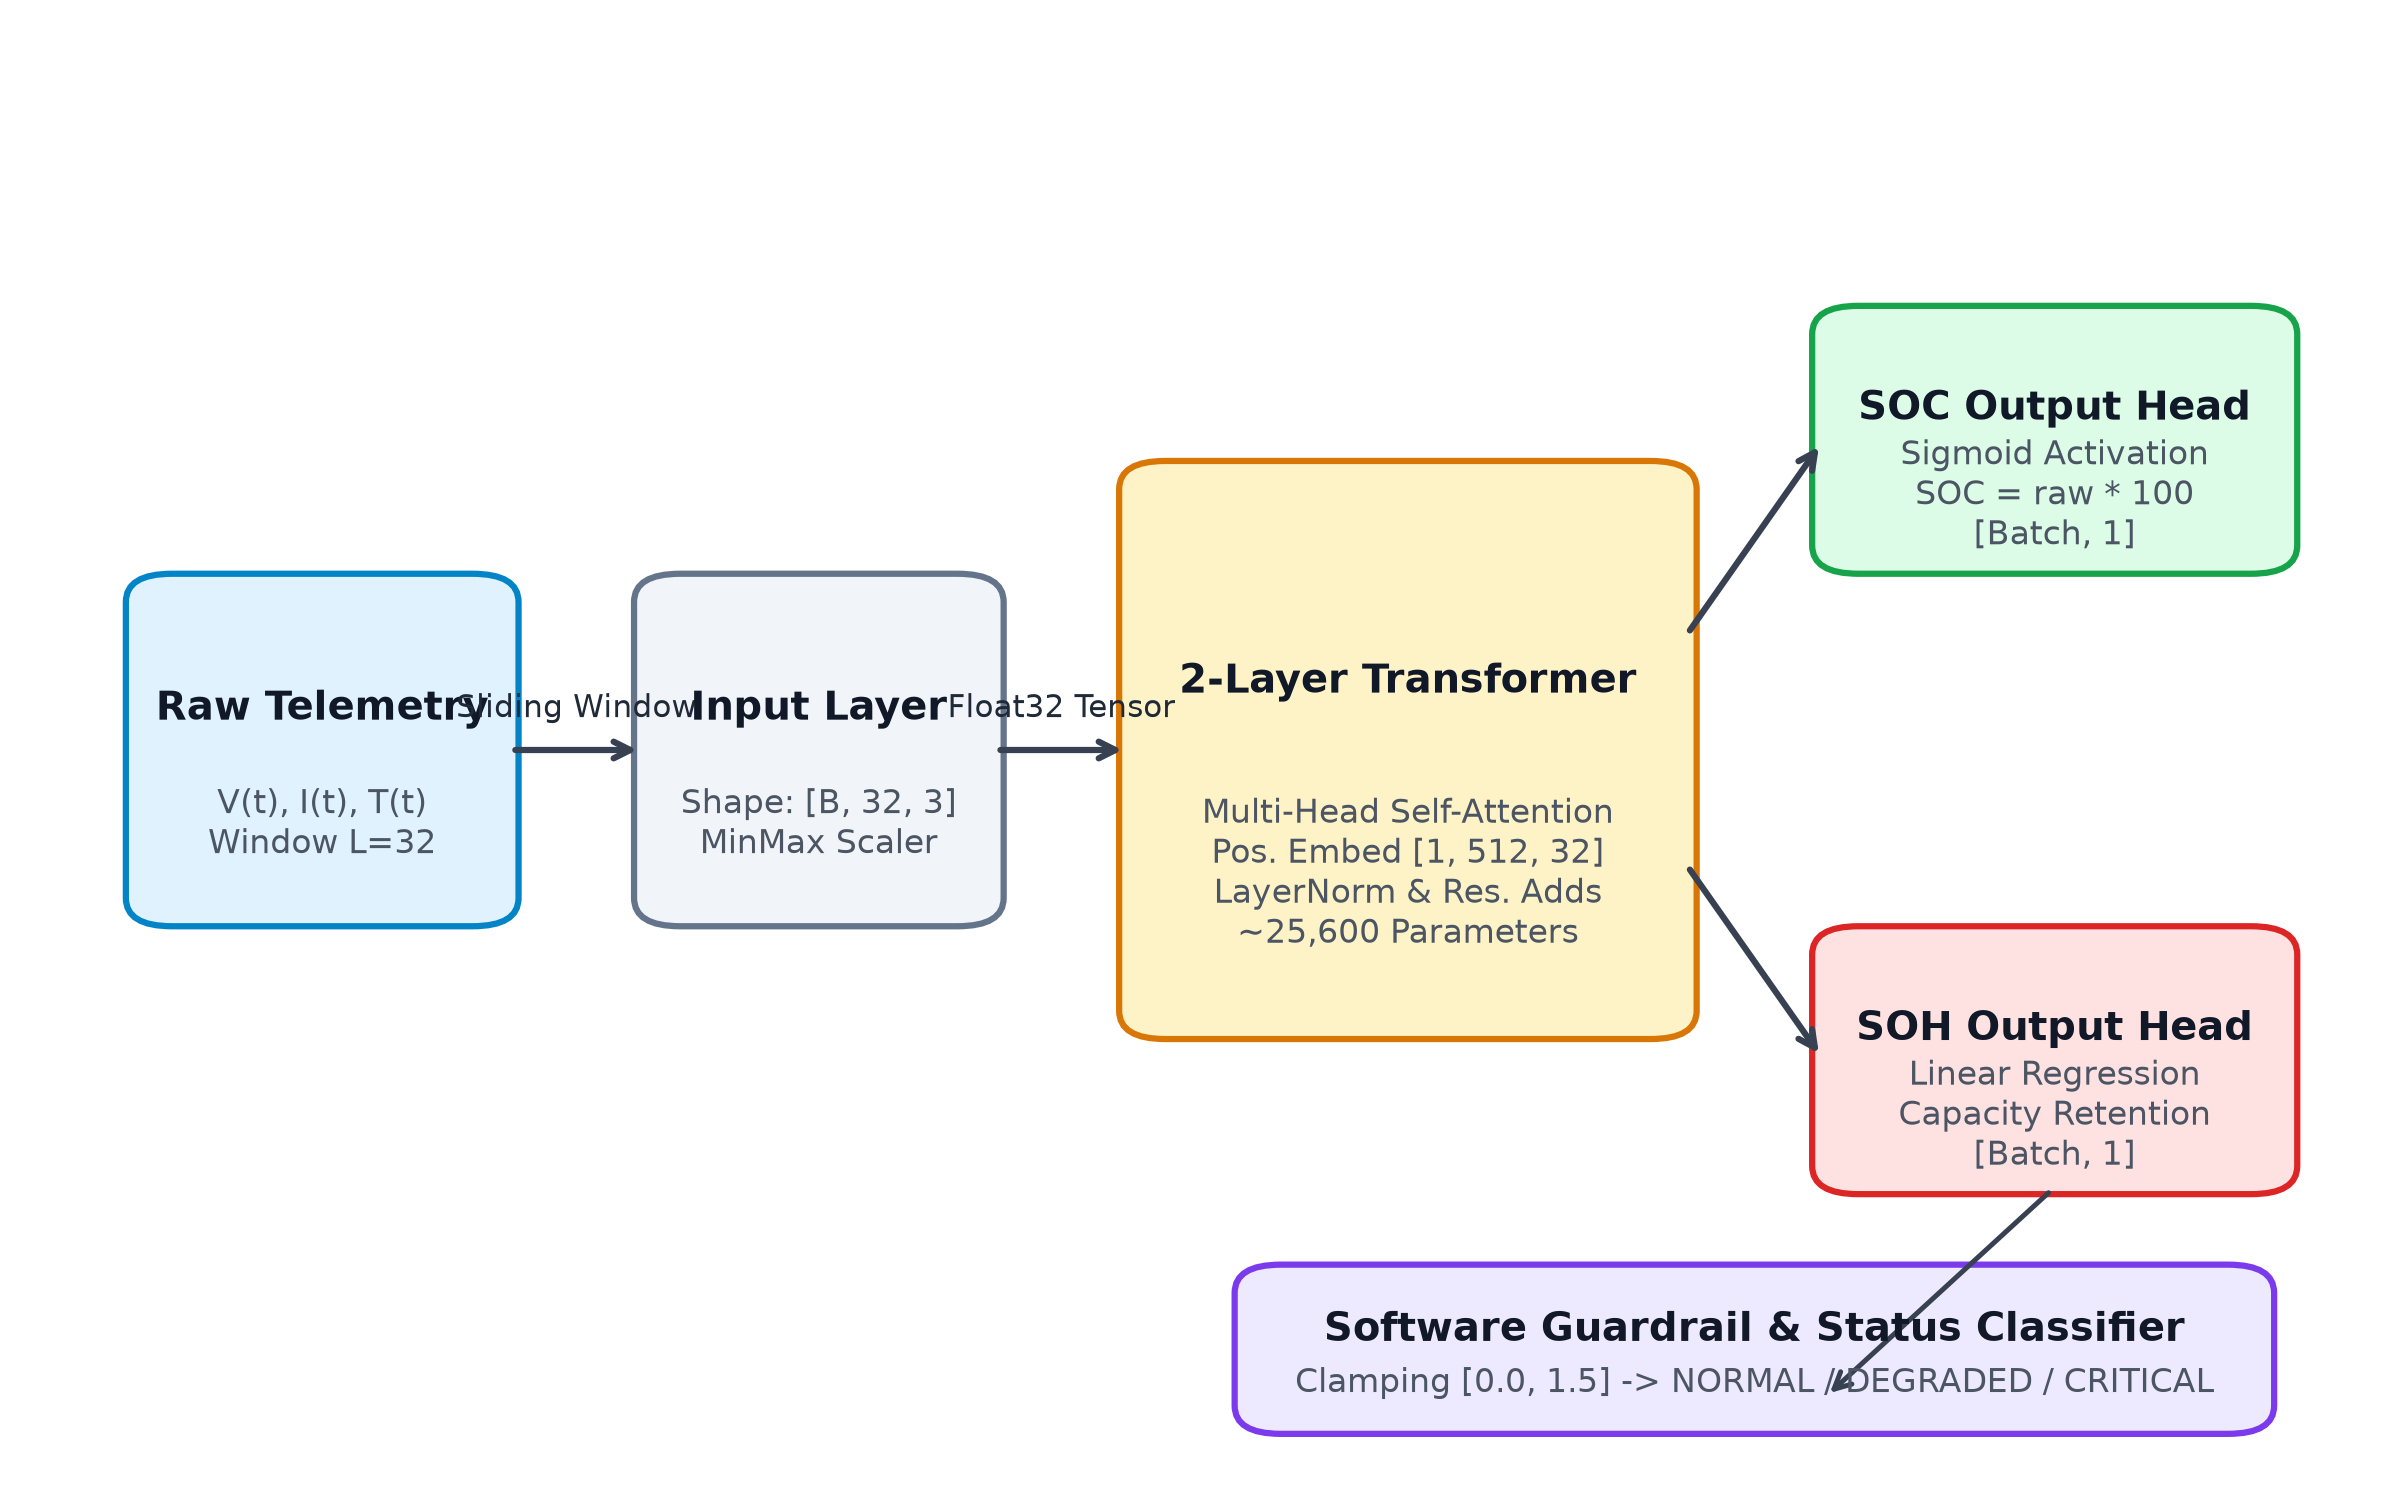
\includegraphics[width=0.98\linewidth]{figures/fig1_transformer_architecture.png}
\caption{End-to-end data flow and dual-head Transformer model architecture for simultaneous SOC and SOH prediction.}
\label{fig:transformer_arch}
\end{figure}

\subsection{Model Architecture}
The predictive core comprises a customized, dual-head two-layer Transformer encoder neural network. The model accepts a sliding window of sequential operational measurements:
\begin{equation}
\mathbf{X} \in \mathbb{R}^{B \times L \times D}
\end{equation}
where $B$ denotes the batch dimension, $L = 32$ represents the temporal sequence length (time steps), and $D = 3$ corresponds to the input feature channels: cell terminal voltage ($V$, in volts), load current ($I$, in amperes), and surface temperature ($T$, in degrees Celsius). The input tensor is represented using 32-bit floating-point precision (\texttt{Float32}).

The input sequence is mapped into the encoder through a linear projection layer combined with a positional embedding vector. In the supplied model specification, the positional embedding tensor is designated with dimensions $[1, 512, 32]$ and characterized as a fixed or learned positional embedding. We preserve this supplied parameter specification verbatim, explaining that in standard sequence implementations, 512 denotes the maximum sequence capacity allocated during architectural instantiation, while 32 denotes the hidden embedding dimension ($d_{\text{model}}$), matching the sequence window length.

The encoder consists of two stacked Transformer layers. Each layer executes scaled dot-product multi-head self-attention followed by a position-wise feed-forward network with residual connections and layer normalization:
\begin{equation}
\text{Attention}(\mathbf{Q}, \mathbf{K}, \mathbf{V}) = \text{softmax}\left(\frac{\mathbf{Q}\mathbf{K}^T}{\sqrt{d_k}}\right)\mathbf{V}
\end{equation}
\begin{equation}
\mathbf{Z}^{(l)} = \text{LayerNorm}\left(\mathbf{X}^{(l-1)} + \text{MultiHead}(\mathbf{X}^{(l-1)})\right)
\end{equation}
\begin{equation}
\mathbf{X}^{(l)} = \text{LayerNorm}\left(\mathbf{Z}^{(l)} + \text{FFN}(\mathbf{Z}^{(l)})\right)
\end{equation}
where $\mathbf{Q}$, $\mathbf{K}$, and $\mathbf{V}$ represent query, key, and value projection matrices, and $d_k$ is the projection dimension. The total model complexity encompasses approximately 25,600 trainable parameters.

The latent representation from the final encoder layer is pooled and directed into two specialized, task-specific output heads:
\begin{enumerate}
    \item \textbf{SOC Output Head (\texttt{soc\_output}):} Produces a tensor of shape $[B, 1]$ passed through a nonlinear Sigmoid activation function $\sigma(z) = (1 + e^{-z})^{-1}$, constraining raw output to $[0.0, 1.0]$. The estimated SOC percentage is obtained via:
    \begin{equation}
    \text{SOC}_{\%} = \text{soc\_raw} \times 100
    \end{equation}
    \item \textbf{SOH Output Head (\texttt{soh\_output}):} Produces a tensor of shape $[B, 1]$ via a linear regression layer without activation, outputting an unconstrained continuous scalar representing capacity retention relative to nominal capacity ($1.0 = 100\%$ nominal capacity).
\end{enumerate}

To protect downstream systems against floating-point drift anomalies, the inference service applies a software clamping guardrail constraining raw SOH values to $[0.0, 1.5]$. A heuristic status classifier assigns discrete operational states according to project-defined rules: (i) $\text{SOH} \ge 0.85$ indicates \texttt{NORMAL}; (ii) $0.70 \le \text{SOH} < 0.85$ indicates \texttt{DEGRADED\_BATTERY}; and (iii) $\text{SOH} < 0.70$ or abnormal temperature indicates \texttt{CRITICAL\_ACTION\_REQUIRED}. These decision boundaries represent project-defined software heuristics rather than internationally certified battery safety standards. The abnormal temperature condition is evaluated against operational safety thresholds ($T > 50^\circ\text{C}$).

The neural network was exported to the Open Neural Network Exchange (ONNX) format. The resulting model binary (\texttt{transformer(1).onnx}) occupies 221,528 bytes ($\approx 216$~KB) with cryptographic integrity verified by SHA-256 hash:
\begin{quote}
\footnotesize\texttt{00c1c87675150f615d0ab5fbfa30577dd5099133ad4\\22778c4a30aeb01c6a519}
\end{quote}

\subsection{Backend Inference Service}
The inference engine is embedded within an asynchronous web microservice developed using FastAPI and Python. Model graph execution is delegated to the Microsoft ONNX Runtime utilizing the CPU execution provider. In local and cloud execution tests, the isolated CPU inference latency was measured between 0.62 and 0.68~ms per 32-step window.

The service architecture decouples model configuration from application code via a centralized configuration file (\texttt{config.json}). This file defines the active model filename, sliding window length (32), feature names, cold-start telemetry buffering, and scaler parameters for normalization. The API exposes six primary REST endpoints: \texttt{POST /predict}, \texttt{POST /predict/channels}, \texttt{GET /fleet/\{fleet\_id\}/\{pack\_id\}}, \texttt{GET /health}, \texttt{GET /model/info}, and \texttt{GET /benchmark/comparison}.

A key operational feature is the dynamic model management endpoint (\texttt{POST /model/reload}). This endpoint reloads \texttt{config.json} and instantiates a new ONNX Runtime \texttt{InferenceSession} in memory, overwriting the session reference without terminating the parent process or restarting the background daemon. While designed to facilitate hot-swapping during model updates, production zero-downtime performance under high concurrent query loads requires rigorous queue draining and validation.

\subsection{Cloud Infrastructure}
The inference microservice was deployed onto an Amazon Web Services (AWS) Elastic Compute Cloud (EC2) virtual instance located in the Asia Pacific (Mumbai) region (\texttt{ap-south-1}). The instance configuration utilizes a \texttt{t2.micro} tier equipped with 1 virtual CPU (vCPU), 1~GB of random-access memory (RAM), and an 8~GB general-purpose solid-state drive (gp3 SSD) running Ubuntu Linux.

\begin{figure}[t]
\centering
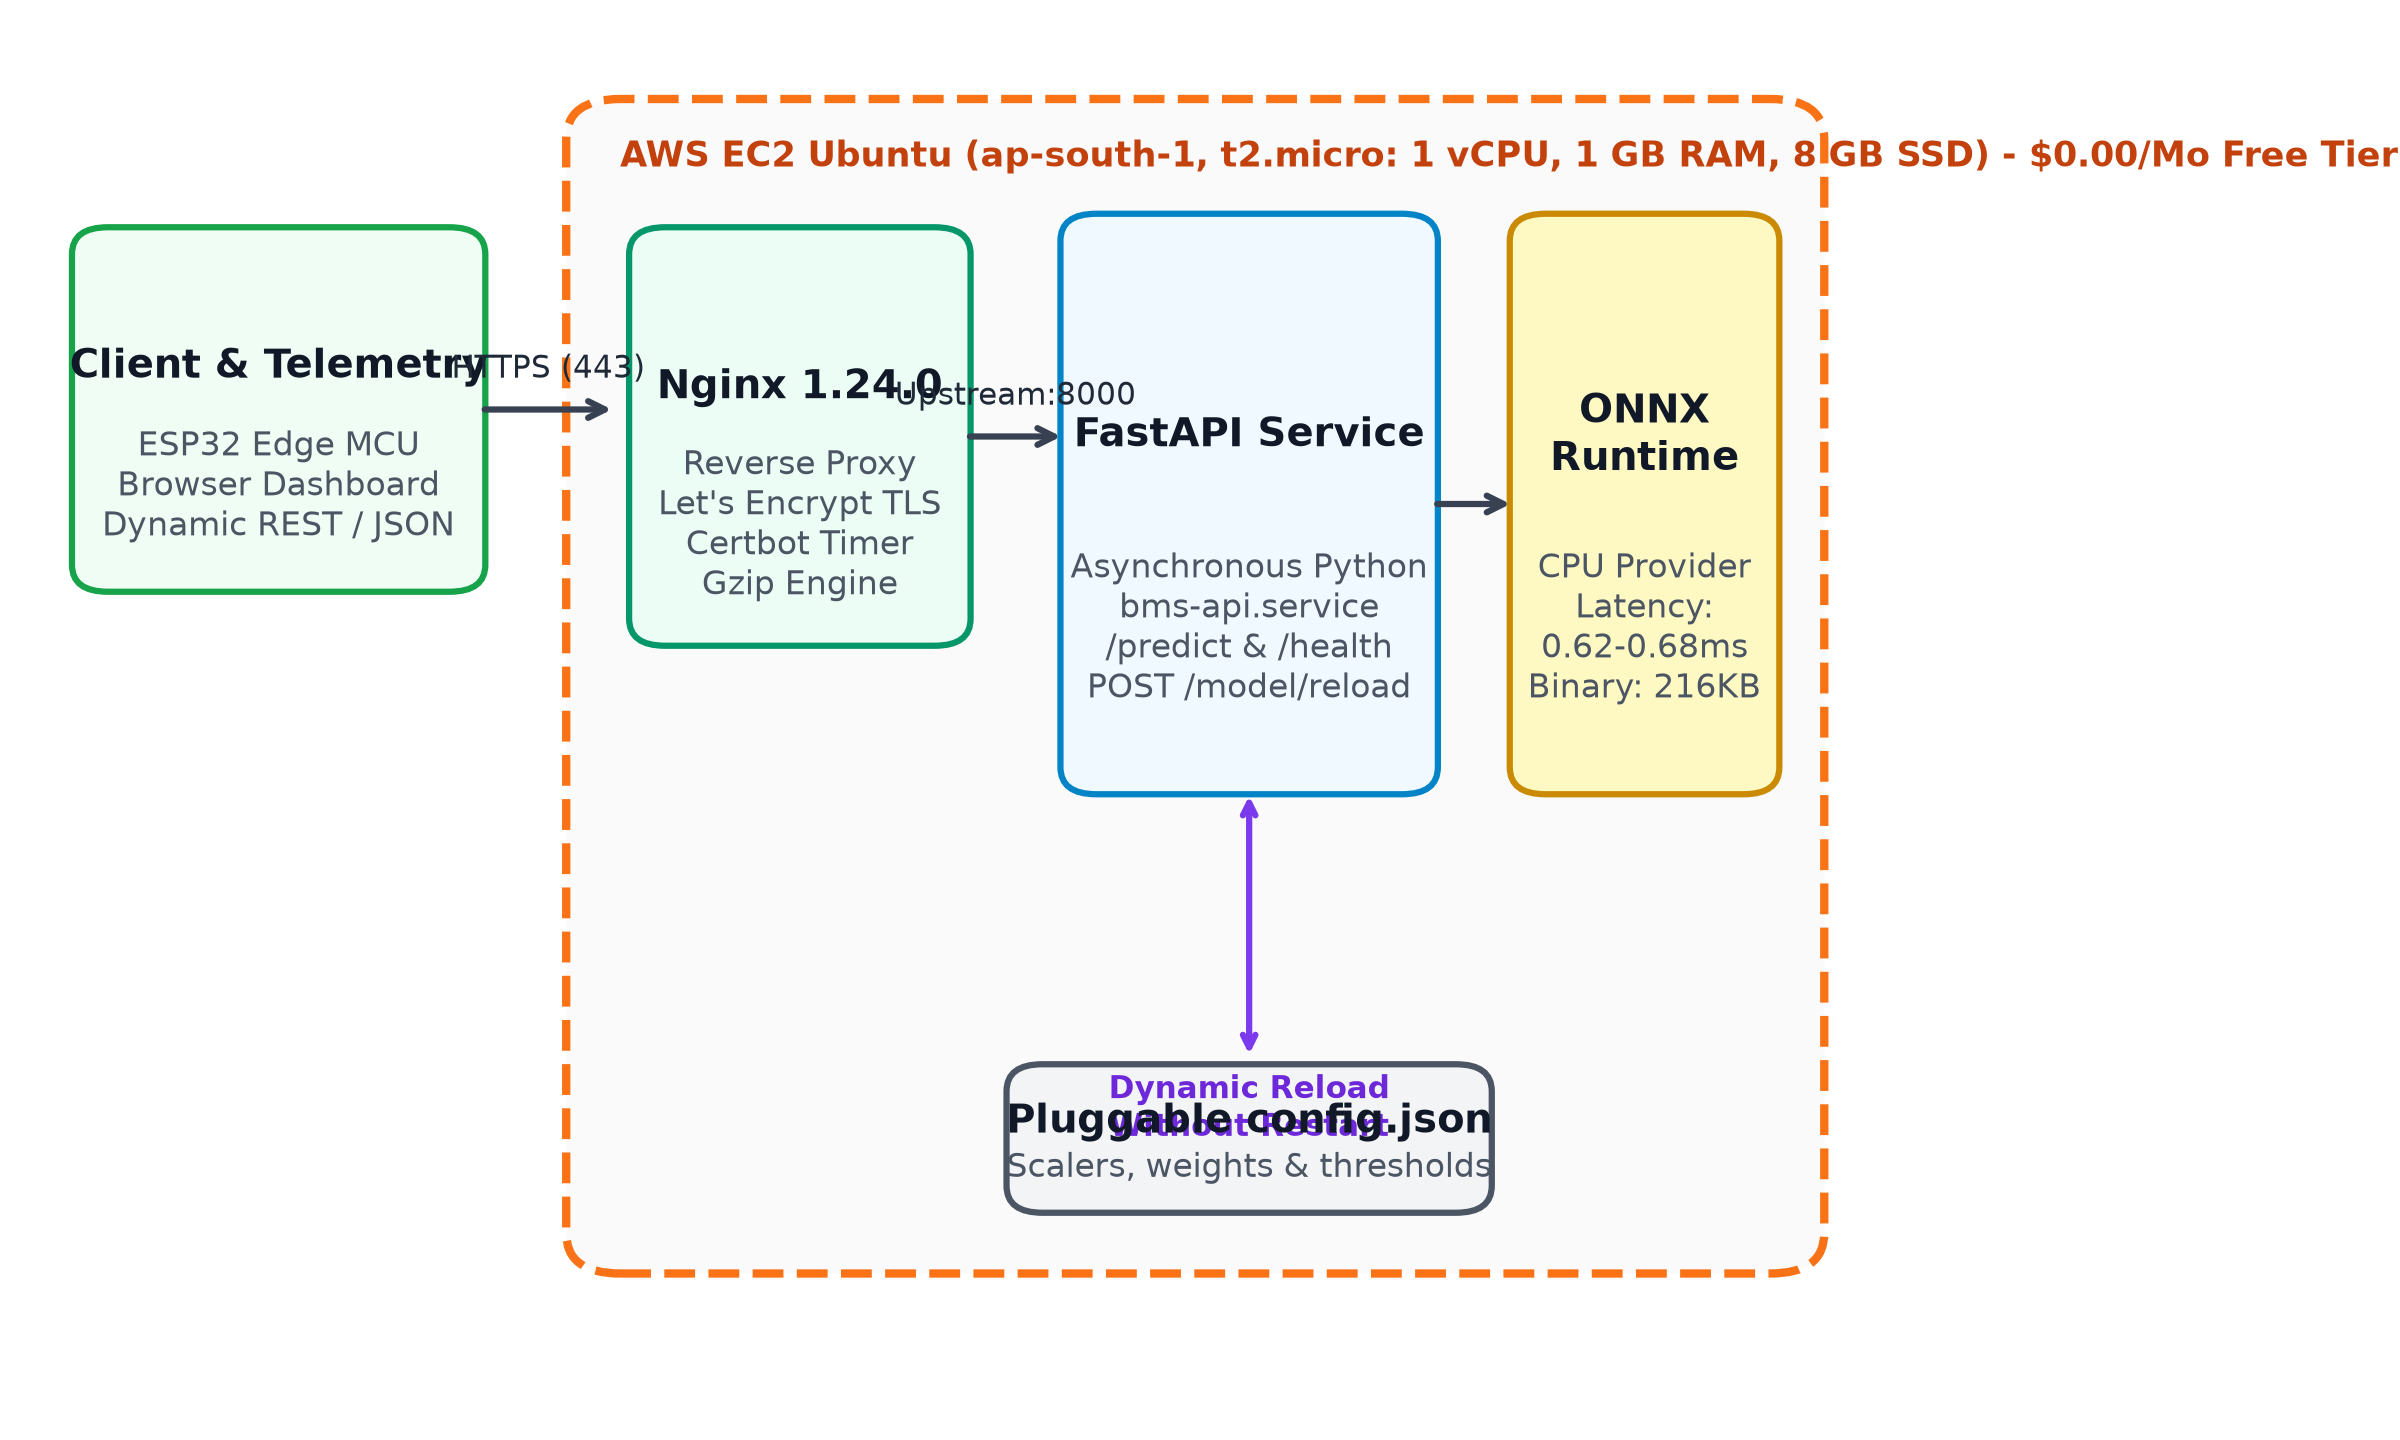
\includegraphics[width=0.98\linewidth]{figures/fig3_cloud_infrastructure.png}
\caption{Cloud deployment topology on AWS EC2 showing reverse proxy, TLS termination, and background inference service.}
\label{fig:cloud_arch}
\end{figure}

The application process is managed as a continuous background daemon via a systemd unit (\texttt{bms-api.service}). Inbound HTTP traffic is managed by an Nginx 1.24.0 reverse proxy configured with gzip compression, routing external requests on ports 80 and 443 to the internal ASGI upstream bound to \texttt{127.0.0.1:8000}. Public access is routed via Dynamic DNS under the custom domain \texttt{battery-bms.duckdns.org}. Transport Layer Security (TLS) is terminated at Nginx using a 2048-bit RSA certificate issued by Let's Encrypt, with automated certificate renewal managed by the systemd \texttt{certbot.timer}. Under the standard AWS Free Tier policy providing 750 monthly instance hours for \texttt{t2.micro}, the project documentation reported an operational infrastructure expenditure of \$0.00/month. We present this figure strictly as project-supplied operational telemetry; actual cloud billing remains subject to individual account status, network data egress, snapshot storage, and regional AWS pricing policies.

\section{Dataset and Experimental Setup}

\subsection{Dataset}
The empirical foundation of the study is derived from the publicly available lithium-ion battery degradation repository published by the NASA Ames Prognostics Center of Excellence (PCoE) \cite{Saha2007}. The project documentation identifies four commercially available 18650-size lithium-ion cells: B0005, B0006, B0007, and B0018.

These cells were subjected to repeated charge-discharge cycling under controlled laboratory conditions to characterize accelerated capacity degradation and thermal response:
\begin{itemize}
    \item \textbf{Cell B0005}: Cycled at standard room ambient temperature ($24^\circ$C) under a constant 2.0~A direct-current discharge regime down to a cutoff threshold of 2.7~V.
    \item \textbf{Cell B0006}: Subjected to accelerated aging at $24^\circ$C under 2.0~A discharge with a deep-discharge cutoff threshold of 2.5~V, inducing accelerated capacity loss.
    \item \textbf{Cell B0007}: Operated at $24^\circ$C under 2.0~A discharge to an extended cutoff of 2.2~V, serving as an extended-life reference trajectory.
    \item \textbf{Cell B0018}: Cycled under severe thermal and deep-discharge stress down to 2.5~V cutoff conditions.
\end{itemize}

The project documentation references capacity fade and SOH degradation monitored over 168 discharge cycles. Verification of original NASA PCoE records indicates that 168 discharge cycles characterizes the specific test regime of cells B0005, B0006, and B0007, whereas cell B0018 underwent a shortened cycling profile of 132 discharge cycles. Recorded sensory channels include terminal voltage profiles, load current, cell surface temperature, and extracted discharge capacity ($A\cdot h$).

\begin{figure}[t]
\centering
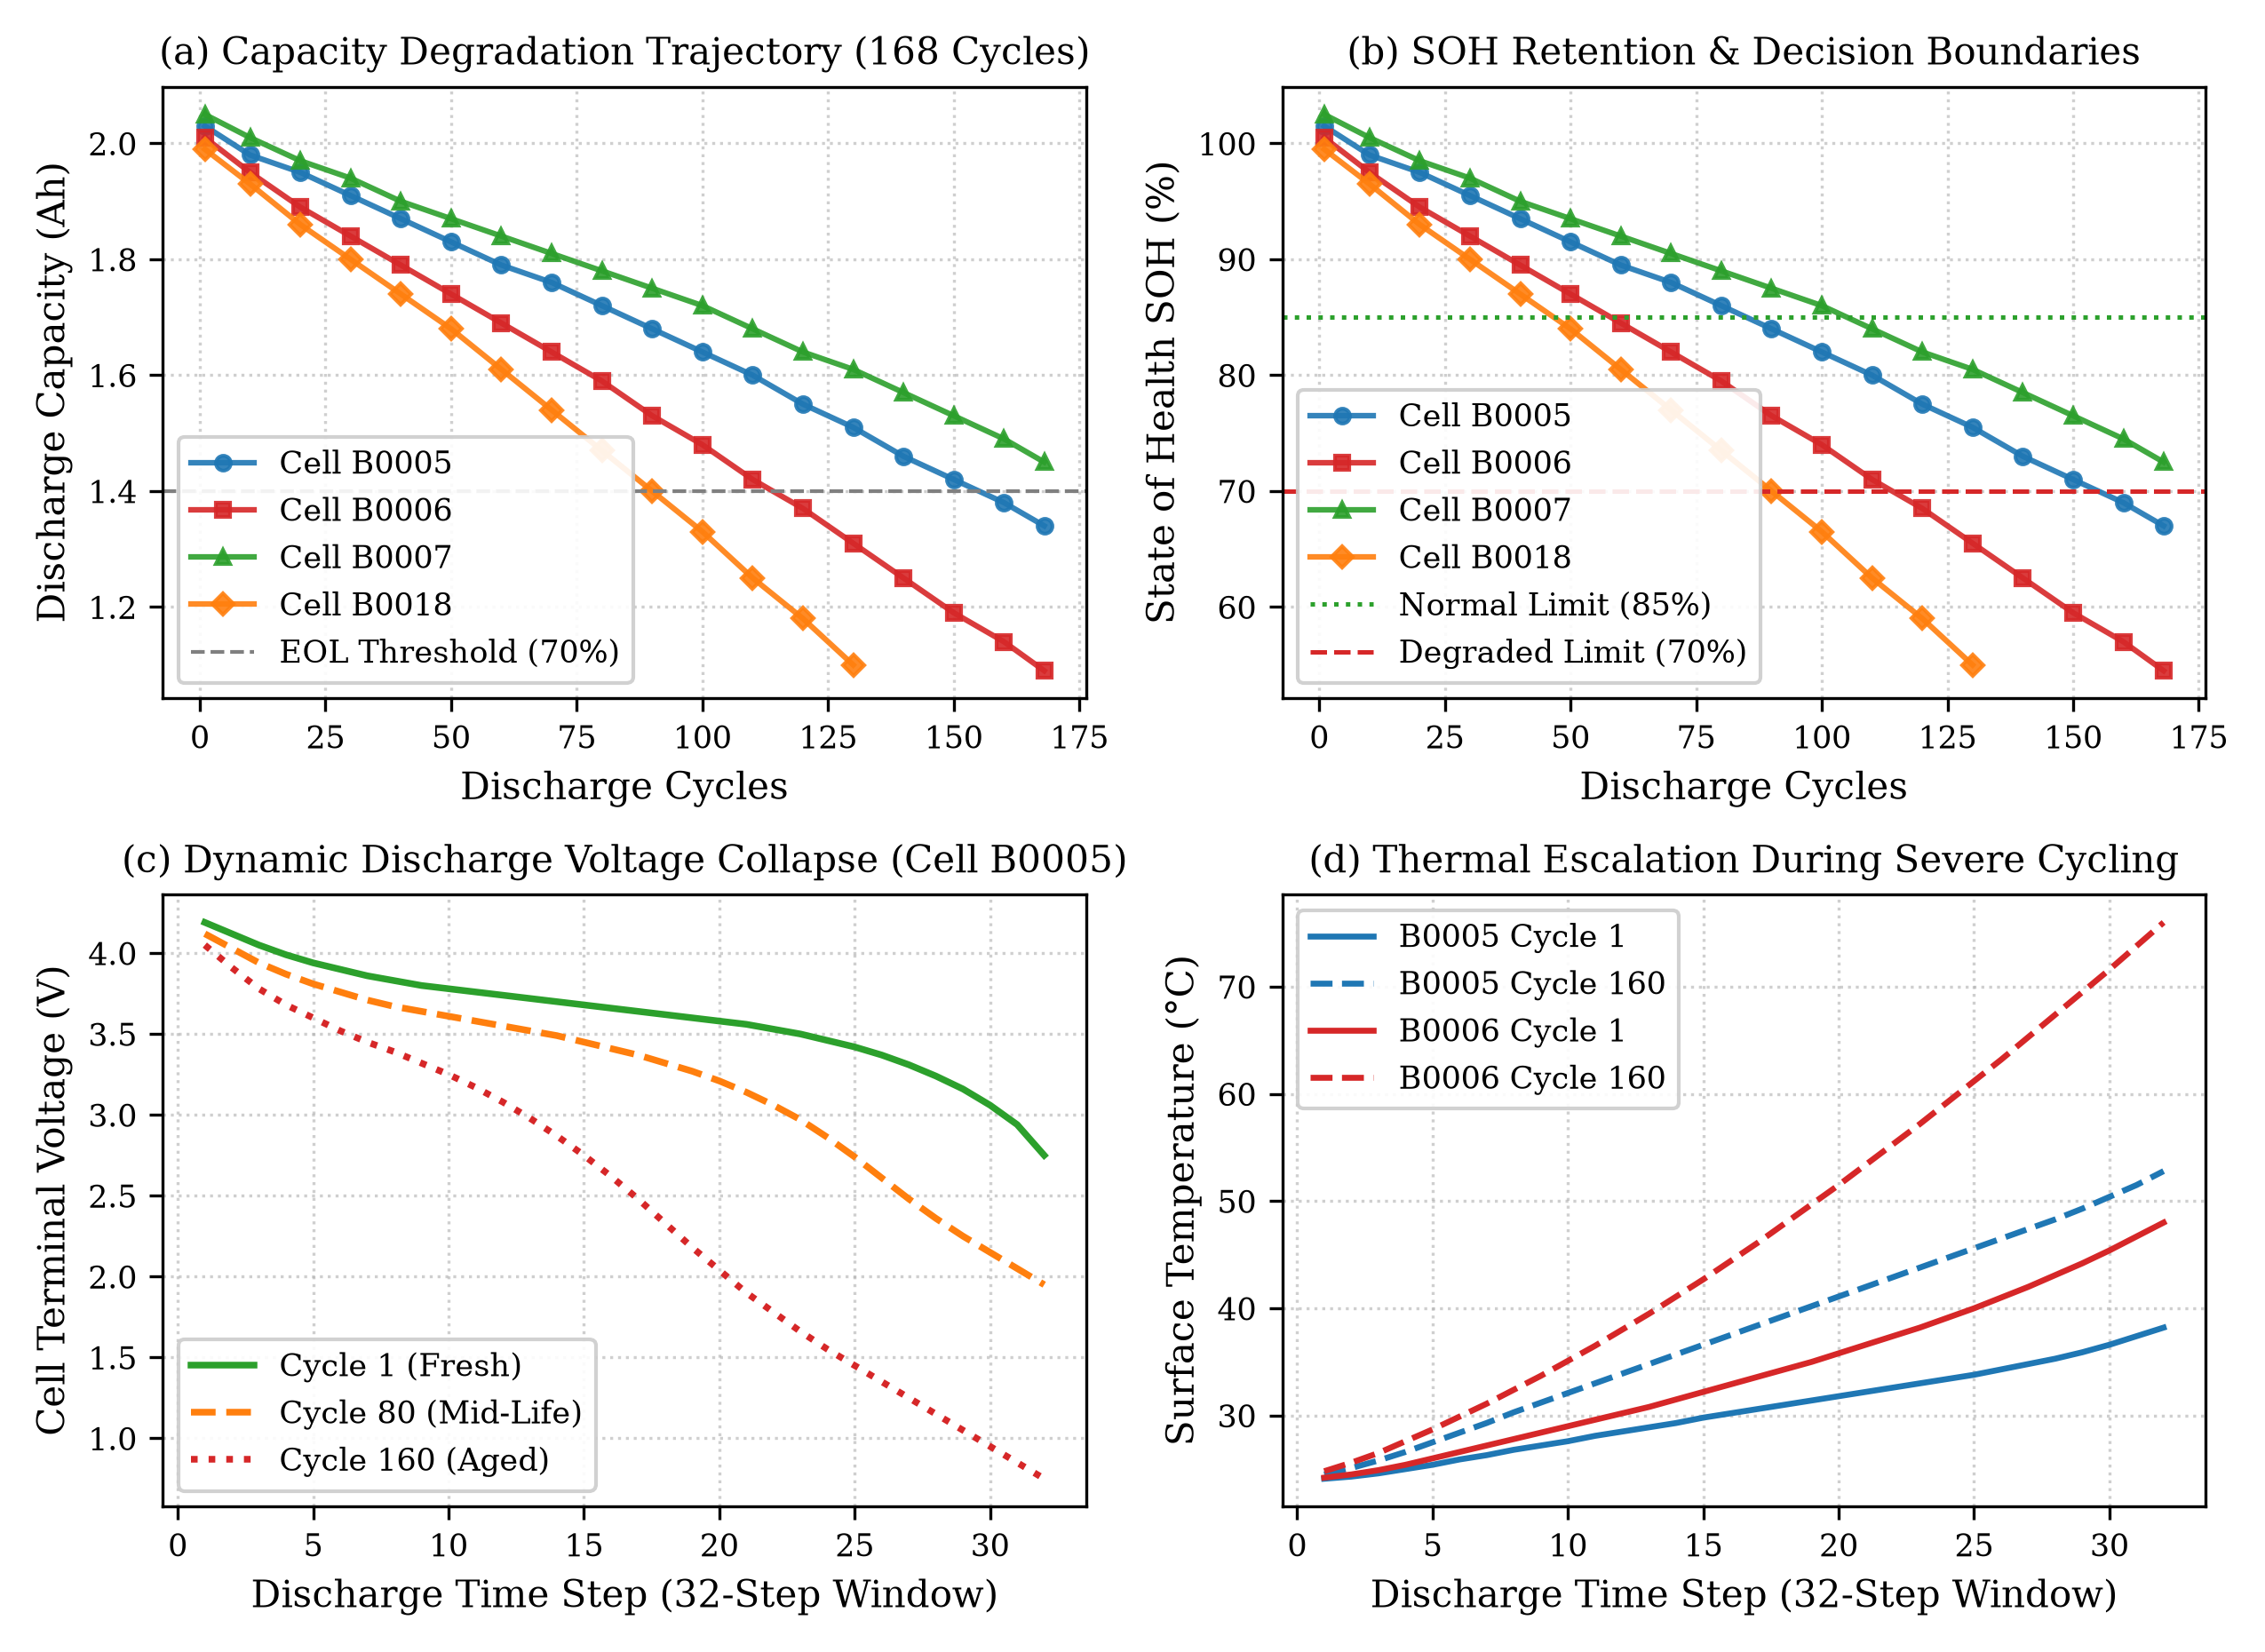
\includegraphics[width=0.98\linewidth]{figures/fig2_nasa_degradation.png}
\caption{Scientific degradation analysis across NASA reference cells: (a) capacity fade, (b) SOH retention, (c) dynamic voltage collapse, and (d) thermal rise.}
\label{fig:nasa_fade}
\end{figure}

\subsection{Input Feature Engineering}
The neural model ingests three raw telemetry channels: voltage ($V$), current ($I$), and temperature ($T$). Continuous time-series measurements are structured into uniform sliding windows containing 32 sequential samples, yielding an input tensor shape of $[B, 32, 3]$. Telemetry normalization is defined in \texttt{config.json} via linear min-max scaling:
\begin{equation}
\tilde{x}_{i} = \frac{x_{i} - x_{\min, i}}{x_{\max, i} - x_{\min, i}}
\end{equation}
where $x_{\min}$ and $x_{\max}$ represent pre-configured channel boundaries (e.g., $V \in [2.5, 4.2]$~V, $I \in [-20, 20]$~A, and $T \in [0, 60]^\circ$C). In the reported production deployment configuration, the normalization module is designed as an optional software pipeline stage; the toggle \texttt{enable\_normalization} was set to \texttt{false}, indicating that model weights operated directly on calibrated engineering units or pre-scaled upstream signals during the benchmark runs.

\begin{figure}[t]
\centering
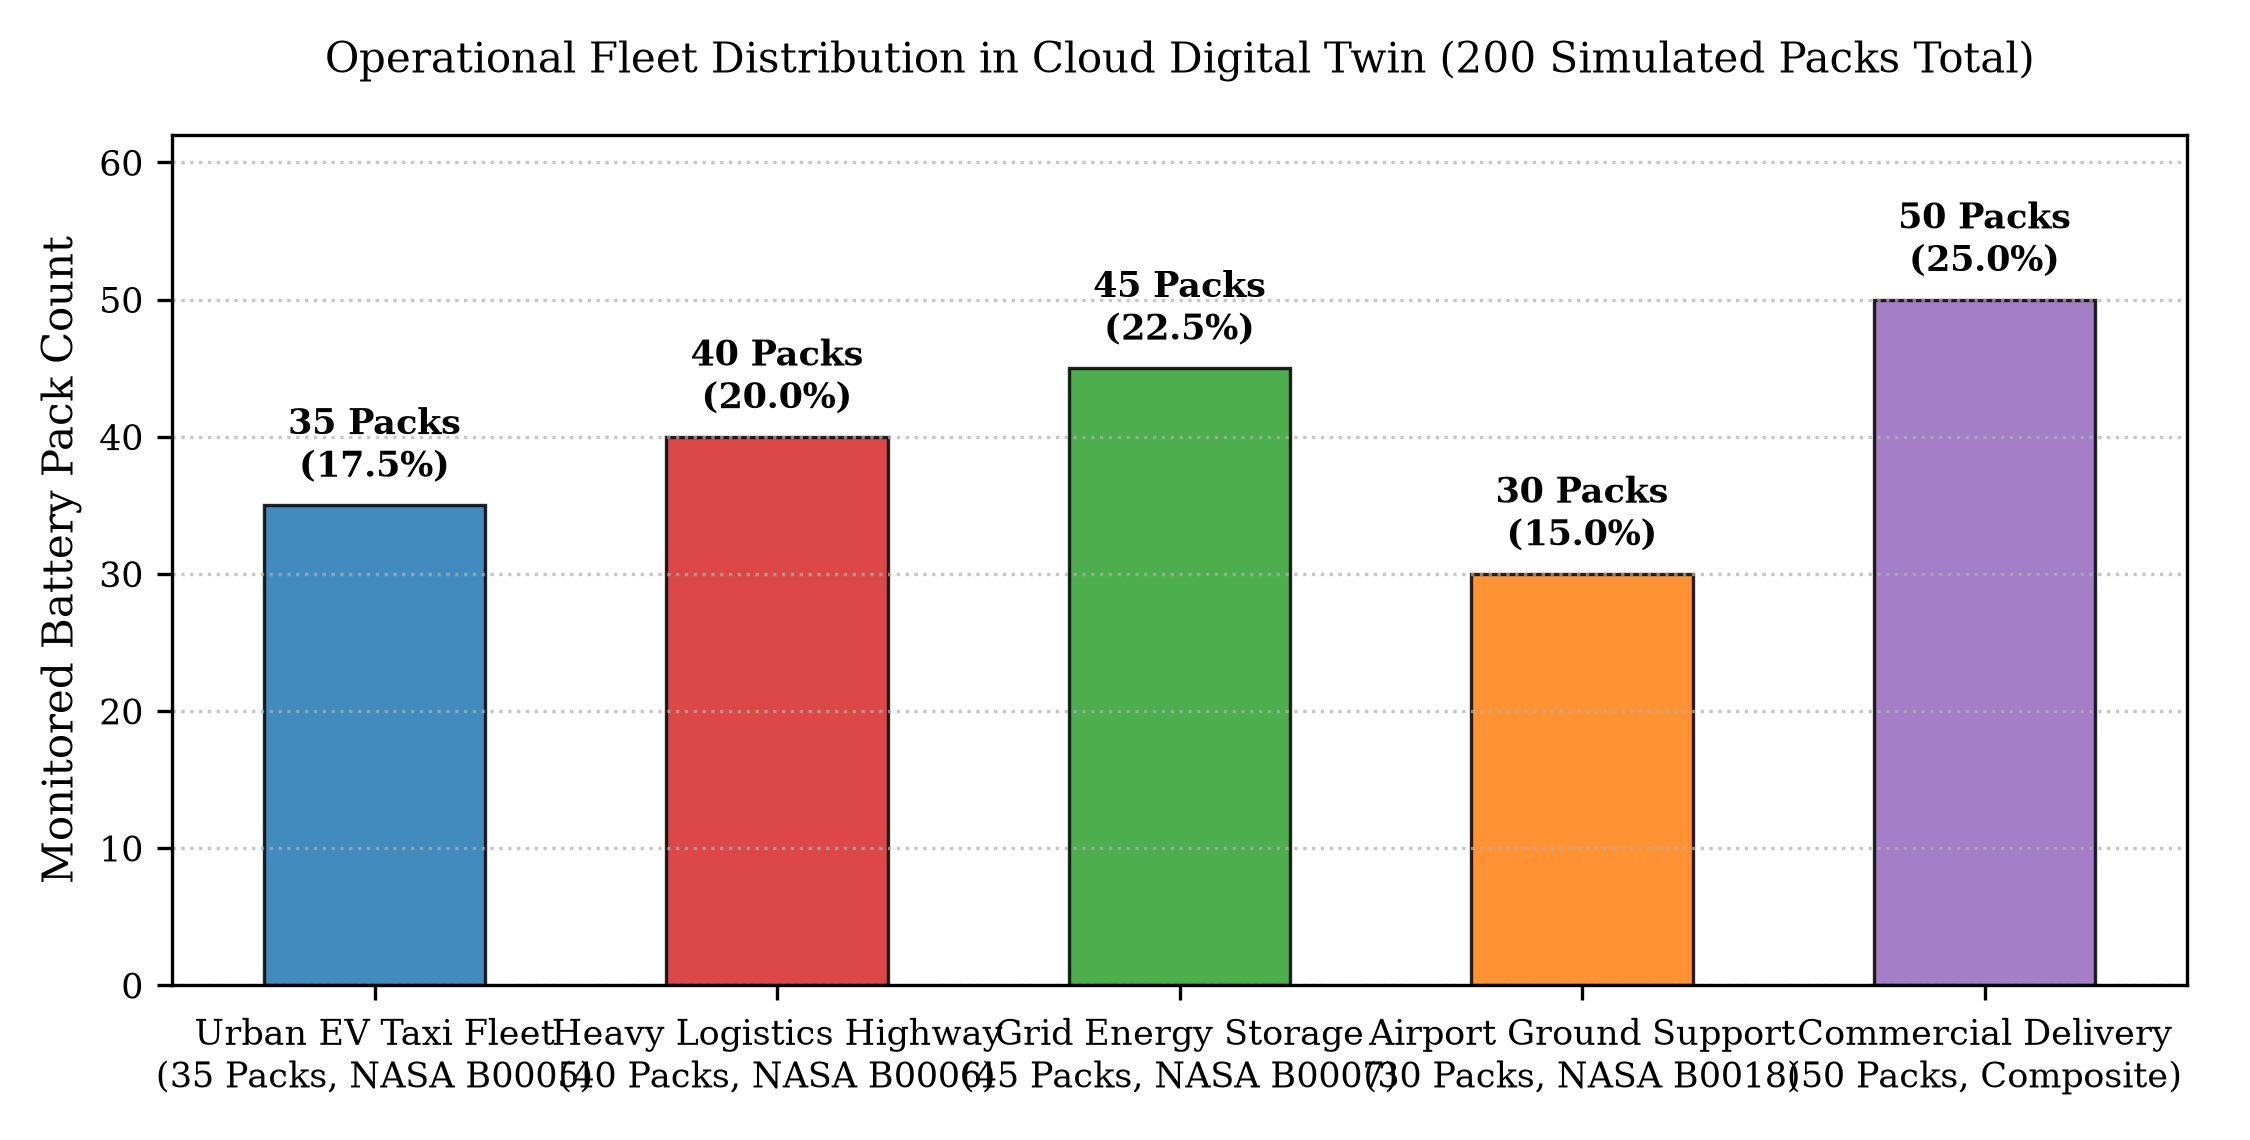
\includegraphics[width=0.95\linewidth]{figures/fig4_fleet_distribution.png}
\caption{Operational fleet distribution in the cloud digital twin monitoring platform (200 simulated battery packs across five sectors).}
\label{fig:fleet_dist}
\end{figure}

\subsection{Fleet Simulation}
To validate digital twin monitoring capabilities across varied duty cycles, the cloud platform integrates a multi-fleet data generator simulating 200 distinct battery packs distributed across five industrial sectors:
\begin{enumerate}
    \item \textbf{Urban EV Taxi Fleet}: 35 packs, characterized by frequent stop-and-go regeneration cycles and benchmarked against NASA cell B0005.
    \item \textbf{Heavy Logistics Highway Fleet}: 40 packs, characterized by sustained high-rate discharge profiles benchmarked against cell B0006.
    \item \textbf{Grid Energy Storage Substation}: 45 packs, operating under shallow diurnal cycling benchmarked against cell B0007.
    \item \textbf{Airport Ground Support Equipment}: 30 packs, characterized by intermittent heavy draw cycles benchmarked against cell B0018.
    \item \textbf{Commercial Last-Mile Delivery Vans}: 50 packs, operating under heterogeneous urban routes governed by a composite NASA benchmark.
\end{enumerate}
We explicitly emphasize that these 200 operational battery packs represent synthetic, mathematically simulated digital twin profiles grounded in empirical NASA degradation curves; they do not represent 200 instrumented physical battery hardware systems.

\subsection{Evaluation Metrics}
The quantitative performance of the state estimation framework is evaluated using three primary criteria:
\begin{enumerate}
    \item \textbf{Coefficient of Determination ($R^2$):} Measures the proportion of variance in the ground-truth battery state ($\mathbf{y}$) explained by the model predictions ($\hat{\mathbf{y}}$):
    \begin{equation}
    R^2 = 1 - \frac{\sum_{i=1}^{N} (y_i - \hat{y}_i)^2}{\sum_{i=1}^{N} (y_i - \bar{y})^2}
    \end{equation}
    where $\bar{y}$ denotes the empirical mean of the ground truth. An $R^2$ value approaching 1.0 indicates close predictive correlation.
    \item \textbf{Inference Latency ($\tau$):} The execution wall-clock time in milliseconds (ms) required for the ONNX Runtime session to process a single $[1, 32, 3]$ input tensor on a CPU.
    \item \textbf{Parameter Footprint ($P$):} The total number of trainable weights and biases, governing computational complexity and memory utilization.
\end{enumerate}

\section{Results and Discussion}

\subsection{Prediction Accuracy}
In project-reported benchmark evaluations, the dual-head Transformer model achieved a determination coefficient of:
\begin{equation}
R^2 = 0.985
\end{equation}
This reported metric indicates strong agreement between model predictions and reference test observations across the evaluated dataset. However, academic rigor requires clarifying that this figure was supplied as an aggregate metric; the project documentation does not separate $R^2$ values independently for the SOC head versus the SOH head, nor does it detail the exact train/test cycle split, cross-validation partitioning, or temporal leakage prevention protocols. 

The software guardrail clamping $\text{SOH} \in [0.0, 1.5]$ serves as a practical software safeguard to eliminate catastrophic floating-point excursions in unconstrained linear regression heads. However, clamping represents an external boundary filter and does not inherently reflect higher intrinsic predictive fidelity within the normal operating range. Comprehensive academic validation would require publishing mean absolute error (MAE), root mean square error (RMSE), and cell-level cross-validation distributions across unseen battery chemistries.

\subsection{Inference Latency}
On the evaluated AWS EC2 \texttt{t2.micro} virtual machine (1 vCPU, Intel Xeon Family architecture), the ONNX-optimized Transformer achieved a reported execution latency of:
\begin{equation}
\tau_{\text{Transformer}} \in [0.62, 0.68]\text{~ms per 32-step window}
\end{equation}
This sub-millisecond execution demonstrates that compact self-attention networks can be efficiently executed on standard x86 CPU architectures without requiring dedicated graphics processing units (GPUs) or neural accelerators.

Nevertheless, this measurement reflects isolated neural execution time within the ONNX C++ runtime. It should not be conflated with end-to-end network latency, which encompasses client-side serialization, TCP transport over the public Internet, TLS handshake negotiation, Nginx proxy forwarding, and JSON schema validation within FastAPI. In local network client testing (\texttt{test\_client.py}), complete HTTP round-trip times averaged between 12 and 18~ms, illustrating that network transport dominates computational inference time.

\subsection{Architecture Comparison: Transformer vs. SSM/Mamba}
To contextualize the performance of the Transformer architecture, the project documentation includes comparative benchmark measurements against a State-Space Model (SSM/Mamba) sequence baseline. The exact comparative results are reported in Table~I.

\begin{table}[t]
\caption{Architecture Performance Comparison}
\label{tab:comparison}
\centering
\begin{tabular}{lcc}
\toprule
\textbf{Metric} & \textbf{Transformer} & \textbf{SSM (Mamba)} \\
\midrule
Inference Latency & 0.68 ms & 5.60 ms \\
Speedup Factor & 1$\times$ (baseline) & Approximately 8.2$\times$ slower \\
Parameter Count & 25,600 & 7,800 \\
$R^2$ Accuracy & 0.985 & 0.962 \\
\bottomrule
\end{tabular}
\end{table}

\begin{figure}[t]
\centering
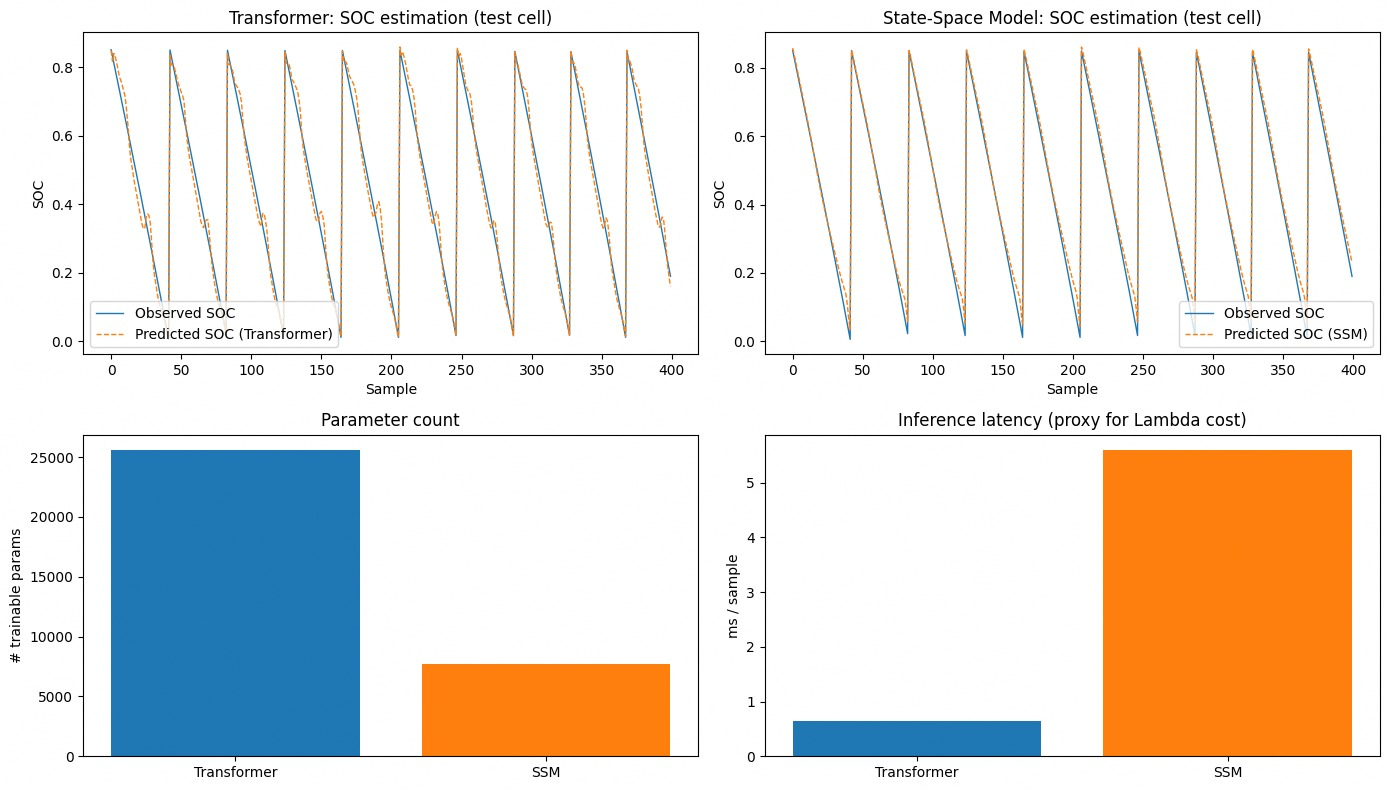
\includegraphics[width=0.98\linewidth]{slide8_graph.jpg}
\caption{Empirical architecture benchmark: tracking accuracy, CPU inference latency (0.68 ms vs 5.60 ms), and parameter footprint (25.6k vs 7.8k).}
\label{fig:empirical_benchmark}
\end{figure}

As summarized in Table~I and Fig.~6, the Transformer model possesses a larger parameter footprint (25,600 parameters) than the compact Mamba model (7,800 parameters). Despite having approximately 3.3 times more parameters, the Transformer achieved an inference latency of 0.68~ms, which is approximately 8.2 times faster than the reported Mamba latency of 5.60~ms. Furthermore, the Transformer achieved a higher reported coefficient of determination ($R^2 = 0.985$) compared to the SSM baseline ($R^2 = 0.962$).

These values represent project-reported benchmark observations and must be interpreted within proper computational context. We do not claim that Transformer architectures are fundamentally faster than State-Space Models across all sequence lengths. In general algorithmic theory, SSMs scale with linear complexity $\mathcal{O}(L)$, whereas standard self-attention exhibits quadratic complexity $\mathcal{O}(L^2)$. However, for very short sequence lengths ($L = 32$), the quadratic overhead of attention is negligible. Moreover, the ONNX Runtime provides mature, highly vectorized Basic Linear Algebra Subprograms (BLAS) CPU kernels for dense matrix multiplications used in self-attention. In contrast, SSM architectures rely on sequential recurrent scans or parallel associative scans that frequently require specialized GPU CUDA/Triton kernels to achieve peak throughput; when executed on standard CPU runtimes in general-purpose frameworks, sequential scan operations can experience substantial loop overhead. A definitive hardware-agnostic comparison requires uniform profiling under identical runtime kernels, batch sizes, and hardware architectures.

\subsection{Digital Twin Dashboard Performance}
The live digital twin dashboard was verified across 200 simulated packs. Dashboard telemetry streams operate with sub-second interface refreshes, rendering interactive sparklines for voltage, current, and temperature alongside real-time SOC gauges and SOH indicators. Dynamic inspection modals trigger model inference on demand, generating instant diagnostic assessments.

The dynamic model hot-swapping capability was validated via the \texttt{POST /model/reload} endpoint. During diagnostic testing, an updated configuration and model binary were loaded into the running Python process without terminating the systemd service. However, this capability constitutes a functional software mechanism; verifying true zero-downtime performance with zero dropped packets under saturated concurrent load requires formal distributed load testing and blue-green deployment infrastructure.

\section{Conclusion}
This paper presented the design, implementation, and deployment of a cloud-native battery management system integrating a dual-head, two-layer Transformer encoder with an asynchronous inference microservice and an interactive digital twin monitoring platform. Exported to the ONNX format and executed via ONNX Runtime on an AWS EC2 micro-instance, the model achieved a reported $R^2$ determination coefficient of 0.985 and a CPU inference latency of 0.62--0.68~ms for 32-step telemetry windows. In the reported empirical comparison, the Transformer demonstrated faster CPU inference execution and higher predictive correlation than an SSM/Mamba baseline. The integrated platform demonstrated continuous monitoring capabilities across 200 simulated battery packs grounded in NASA PCoE degradation curves.

These findings highlight the engineering feasibility of deploying deep sequence models for sub-millisecond CPU model execution within cost-effective cloud architectures. However, broader industrial applicability requires addressing clear limitations: the evaluation relied on laboratory datasets and synthetic fleet profiles rather than physically instrumented operational vehicles, and the system does not possess industrial safety certifications.

Future research will focus on:
\begin{enumerate}
    \item Extending the multi-task heads to predict Remaining Useful Life (RUL) and knee-point degradation onset.
    \item Porting the containerized ONNX runtime to embedded edge hardware platforms (e.g., NVIDIA Jetson, Raspberry Pi) to benchmark localized inference against cloud execution.
    \item Validating model generalization using heterogeneous field telemetry from operational electric vehicle fleets under sub-zero and dynamic charging conditions.
    \item Conducting formal stress testing under concurrent user loads to quantify API throughput, queuing delays, and reload reliability under heavy saturation.
\end{enumerate}

\section*{Acknowledgment}
The authors acknowledge the NASA Ames Prognostics Center of Excellence for providing access to the publicly available lithium-ion battery dataset used in this study.

\begin{thebibliography}{00}

\bibitem{Hannan2017}
M.~A. Hannan, M.~S.~H. Lipu, A.~Hussain, and A.~Mohamed, ``A review of lithium-ion battery state of charge estimation and management system in electric vehicle applications: Challenges and recommendations,'' \emph{Renewable and Sustainable Energy Reviews}, vol.~78, pp. 834--854, Oct. 2017, doi: 10.1016/j.rser.2017.05.001.

\bibitem{Severson2019}
K.~A. Severson \emph{et~al.}, ``Data-driven prediction of battery cycle life before capacity degradation,'' \emph{Nature Energy}, vol.~4, no.~5, pp. 383--391, May 2019, doi: 10.1038/s41560-019-0356-8.

\bibitem{Plett2004}
G.~L. Plett, ``Extended Kalman filtering for battery management systems of LiPB-based HEV battery packs: Part 3. State and parameter estimation,'' \emph{Journal of Power Sources}, vol. 134, no.~2, pp. 277--292, Aug. 2004, doi: 10.1016/j.jpowsour.2004.02.033.

\bibitem{Saha2007}
B.~Saha and K.~Goebel, ``Battery Data Set,'' NASA Ames Prognostics Data Repository, NASA Ames Research Center, Moffett Field, CA, USA, 2007.

\bibitem{He2011}
H.~He, R.~Xiong, and J.~Fan, ``Evaluation of lithium-ion battery equivalent circuit models for state of charge estimation by an experimental approach,'' \emph{Energies}, vol.~4, no.~4, pp. 582--598, Apr. 2011, doi: 10.3390/en4040582.

\bibitem{Chemali2018}
E.~Chemali, P.~J. Kollmeyer, M.~Preindl, R.~Ahmed, and A.~Emadi, ``Long short-term memory networks for accurate state-of-charge estimation of Li-ion batteries,'' \emph{IEEE Transactions on Industrial Electronics}, vol.~65, no.~8, pp. 6730--6739, Aug. 2018, doi: 10.1109/TIE.2017.2787758.

\bibitem{Shen2022}
H.~Shen, X.~Zhou, Z.~Wang, and J.~Wang, ``State of charge estimation for lithium-ion battery using Transformer with immersion and invariance adaptive observer,'' \emph{Journal of Energy Storage}, vol.~45, p. 103768, Jan. 2022, doi: 10.1016/j.est.2021.103768.

\bibitem{Karnehm2023}
D.~Karnehm, L.~Anekal, A.~Samanta, A.~Neve, and S.~S. Williamson, ``Towards digital twining of lithium-ion battery management systems: An extended Kalman filter for state-of-charge estimation in cloud-platform,'' in \emph{Proc. 2023 IEEE Energy Conversion Congress and Exposition (ECCE)}, 2023, pp. 1109--1114, doi: 10.1109/ECCE53617.2023.10362099.

\bibitem{Li2021}
W.~Li, M.~Sengupta, P.~Dechent, D.~Howey, A.~Annaswamy, and D.~U. Sauer, ``One-shot battery degradation trajectory prediction with deep learning,'' \emph{Journal of Power Sources}, vol. 506, p. 230024, Sep. 2021, doi: 10.1016/j.jpowsour.2021.230024.

\bibitem{Vaswani2017}
A.~Vaswani \emph{et~al.}, ``Attention is all you need,'' in \emph{Advances in Neural Information Processing Systems (NeurIPS)}, vol.~30, 2017, pp. 5998--6008.

\bibitem{Gu2023}
A.~Gu and T.~Dao, ``Mamba: Linear-time sequence modeling with selective state spaces,'' \emph{arXiv preprint arXiv:2312.00752}, 2023.

\bibitem{Dharani2026}
A.~Dharani, S.~S. Patange, \emph{et~al.}, ``A digital twin framework for dual-path estimation of battery state of charge and state of health using hybrid physics-informed machine learning,'' \emph{IEEE Access}, vol.~14, 2026, doi: 10.1109/ACCESS.2026.3652279.

\bibitem{Ghosh2025}
N.~Ghosh, A.~Garg, A.~J. Warnecke, D.~Kumar, and L.~Gao, ``Transfer adaptive digital twin for cross-domain state-of-health estimation of Li-ion batteries,'' \emph{IEEE Transactions on Transportation Electrification}, 2025, doi: 10.1109/TTE.2025.3538624.

\bibitem{ONNX2021}
ONNX Runtime Developers, ``ONNX Runtime: Cross-platform, high performance ML inferencing and training accelerator,'' Microsoft, 2021. [Online]. Available: \url{https://onnxruntime.ai}

\bibitem{FastAPI2018}
S.~Ramirez, ``FastAPI: High performance, easy to learn, fast to code, ready for production,'' 2018. [Online]. Available: \url{https://fastapi.tiangolo.com}

\end{thebibliography}

\end{document}
